\documentclass{article}
\usepackage[utf8]{inputenc}
\usepackage[russian]{babel}
\usepackage{graphicx}
\usepackage{amsmath}
\usepackage{breqn}
\usepackage{wrapfig}
\usepackage{float}
\usepackage{multirow}
\usepackage{caption}
\usepackage{subcaption}

\graphicspath{ {./data/images} }
\author{Александр Романов Б01-107}
\date{}
\title{1.2 Исследование эффекта Комптона}

\begin{document}
\maketitle
\section{Введение}
\subsection{О работе}
С помощью сцинтилляционного спектрометра исследуется энергетический спектр \(\gamma\)-квантов, рассеяных на
графите. Определяется энергия рассеянных \(\gamma\)-квантов в зависимости от угла рассеяния, а также энергия
покоя частиц, на которых происходит комптоновское рассеяние.
\subsection{Теоретическая справка}
Пусть электрон до сооударения покоился, а \(\gamma\)-квант имел начальную энергию \(\hbar\omega_0\) и импульс
\(\hbar\omega_0/c\). После соударения электрон приобрёл энергию \(\gamma mc^2\) и импульс \(\gamma mv\), где
\(\gamma = (1-\beta^2)^{-1/2},\; \beta = v/c\), а \(\gamma\)-квант рассеивается на некоторый угол \(\theta\).

Запишем ЗСЭ и ЗСИ:
\[ mc^2 + \hbar\omega_0 = \gamma mc^2 + \hbar\omega_1 \]
\[ \frac{\hbar\omega_0}{c} = \gamma mv\cos{\phi} + \frac{\hbar\omega_1}{c}\cos{\theta} \]
\[ \gamma mv\sin{\phi} = \frac{\hbar\omega_1}{c}\sin{\theta} \]
Решив эту систему:
\[ \Delta\lambda = \lambda_1 - \lambda_0 = \frac{h}{mc}(1-\cos{\theta}) = \Lambda_K (1 - \cos{\theta})\]
где комптоновская длина волны электрона
\[ \Lambda_K = \frac{h}{mc} = 2.42\cdot 10^{-10}\; cm \]
Преобразуем это выражение от длин волн к энергии \(\gamma\)-квантов:
\[ \frac{1}{\varepsilon\left(\theta\right)} - \frac{1}{\varepsilon_0} = 1 - \cos{\theta} \]

\subsection{Экспериментальная установка}
\begin{figure}[H]
  \centering
  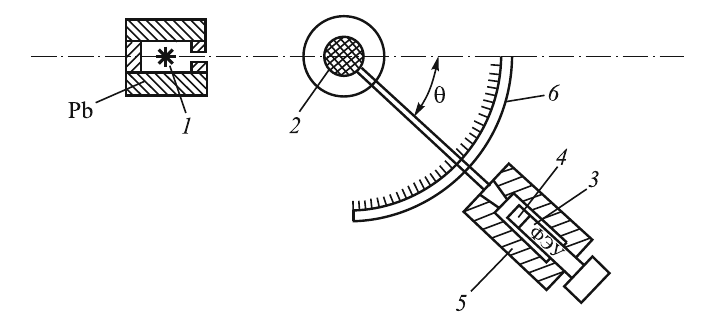
\includegraphics[width=0.8\textwidth]{scheme.png}
	\caption{Блок-схема установки по изучению рассения \(\gamma\)-квантов}
\end{figure}
Заменим энергию на номер канала
\[ \frac{1}{N\left(\theta\right)} - \frac{1}{N\left(0\right)} = A(1-\cos{\theta}) \]
Тогда получим
\[mc^2\left(\frac{1}{E(90)} - \frac{1}{E(0)}\right) = 1\]
Отсюда
\begin{equation}
	mc^2 = E_{\gamma}\frac{N(90)}{N(0) - N(90)} \label{eq:calm}
\end{equation}
\section{Работа}
Включим все измерительные приборы и компьютер.
Запустим программу и войдём в режим измерения спектра. Проверим функциональность.
Будем устанавливать сцинтилляционный счётчик под разными углами \(\theta\) к первоначальному направлению
полёта \(\gamma\)-квантов, снимать амплитудные спектры и определять положения фотопиков для каждого значения
угла \(\theta\).

\begin{table}[!ht]
    \centering
    \begin{tabular}{|c|c|c|c|}
    \hline
				\(\lambda_{l}\), \(channel \#\) & \(\lambda_{r}\), \(channel \#\) & \(\theta,\; \circ\) & \(\lambda_{av},\; channel \#\) \\ \hline
        631 & 663 & 0 & 647 \\ \hline
        550 & 566 & 10 & 558 \\ \hline
        477 & 515 & 20 & 496 \\ \hline
        538 & 561 & 30 & 549.5 \\ \hline
        415 & 451 & 40 & 433 \\ \hline
        361 & 402 & 50 & 381.5 \\ \hline
        306 & 339 & 60 & 322.5 \\ \hline
        278 & 305 & 70 & 291.5 \\ \hline
        256 & 279 & 80 & 267.5 \\ \hline
				224 & 248 & 90 & 236 \\ \hline
        211 & 227 & 100 & 219 \\ \hline
        193 & 208 & 110 & 200.5 \\ \hline
        184 & 196 & 120 & 190 \\ \hline
		\end{tabular}
\end{table}

Построим график \(\frac{1}{N\left(\theta\right)}\) от \(1-\cos{\theta}\)
\begin{figure}[H]
  \centering
  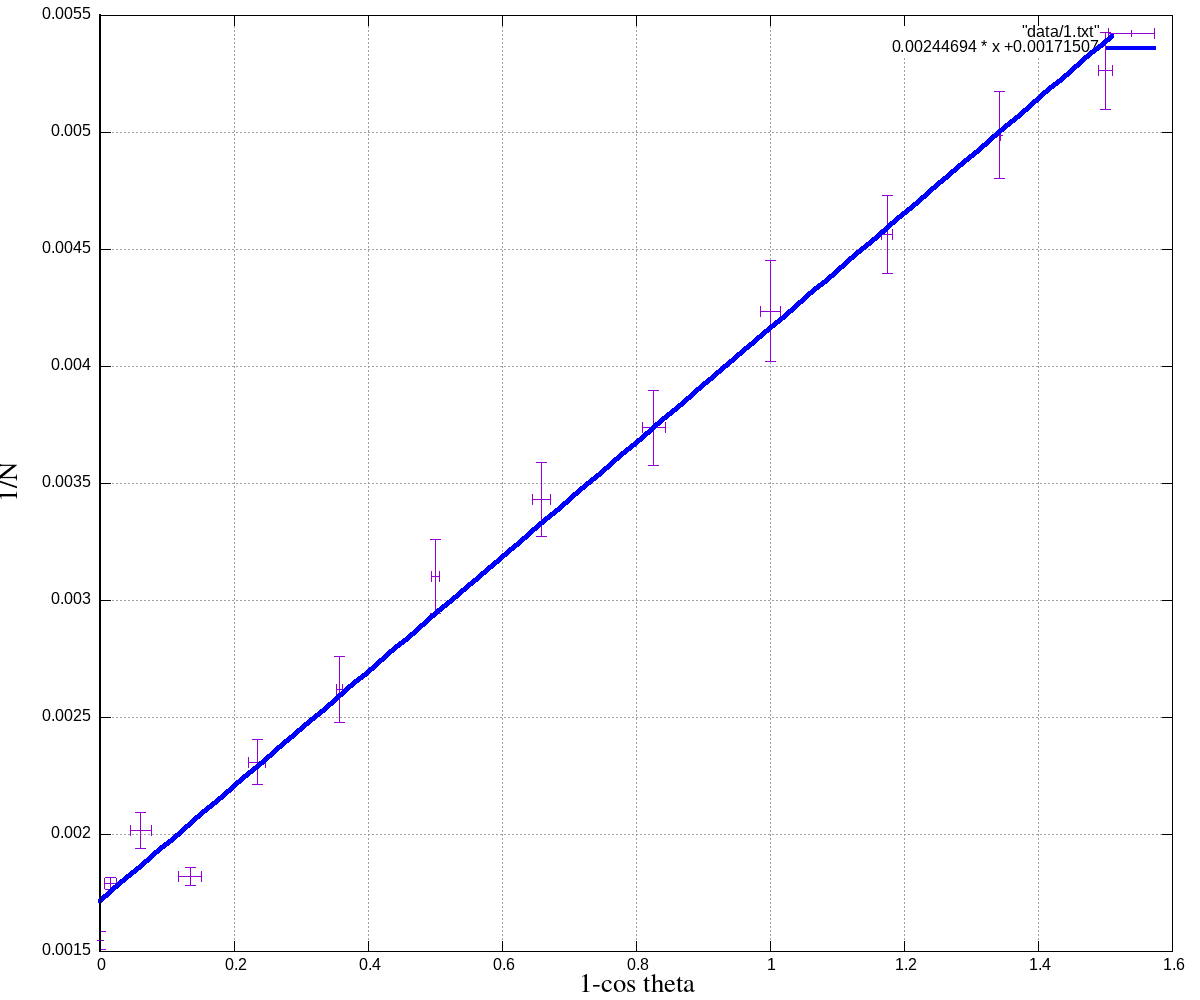
\includegraphics[width=0.8\textwidth]{1.png}
	\caption{График \(\frac{1}{N\left(\theta\right)}\) от \(1-\cos{\theta}\)}
\end{figure}
Получили зависимость вида \(y = kx + b\):
\[ k = 0.00243 \pm 6\cdot 10^{-5}\]
\[ b = 0.0017 \pm 3\cdot 10^{-5} \]
\section{Обработка результатов}
Найдём энергию покоя электрона из формулы (\ref{eq:calm})
\[ mc^2 = E_{\gamma}\frac{\frac{1}{b + k (1-\cos{90})}}{\frac{1}{b + k(1-\cos{0})} - \frac{1}{b + k(1-\cos{90})}} = 460 \text{КэВ}\]
Полученное значение достаточно точно совпадает с теоретическим (\(mc^2 = 500\) КэВ)
\section{Выводы}
В ходе выполнения работы:
\begin{enumerate}
\item С помощью сцитилляционного спектрометра был исследован спектр \(\gamma\)-квантов рассеяных на графите.
\item Было вычесленно значение энергии покоя электрона (460 КэВ). Значение достаточно точно совпадает с теоретическим (500 КэВ)
\end{enumerate}
\end{document}
